\chapter{Results} % Chapter title

\label{chapter:results} % For referencing the chapter elsewhere, use \ref{chapter:computational_neuro} 

\def \resultboxplot {0.8}
%----------------------------------------------------------------------------------------

\section{Multiple Query Optimization}
\label{chapter:results_mqo}

The non-ML circuit as well as the ML optimized one are run on the simulator as well as on real hardware. For this, the IBM Falcon r4L processor \code{ibmq\_bogota v1.6.37} is used. Each circuit runs 13 times, and the parity function referenced in the chapter \todo{add reference to parity explanation} is used for the ML optimized circuit as well as the non-ML circuit to allow for a direct comparison. For direct comparison, both the ML and non-ML circuit are evaluated using filtered and parity evaluation. The runs are made on a problem space $\left|\mathcal{D}_{2\times2}\right| =\ 300$, out of which 25\%, so 75 records, are taken and evaluated. These 75 records are the same used in the evaluation of the ML optimized circuit in chapter \ref{chapter:mqo_machine_learning}. The results are shown in figures \ref{figure:comparison_ml_noml_filtered_acc} - \ref{figure:ml_rhw_dist}.

\begin{figure}[!h]
    \centering
    \scalebox{\resultboxplot}{
        \includesvg{thesis/Appendices/comparison_ml_noml_circuit_filtered_acc.svg}
    }
    \caption{Direct comparison of the non-ML and ML circuits in terms of accuracy, once on the simulator (annotated with SIM) and once on real hardware (annotated with RHW). The accuracy is determined by the amount of best combinations the circuit evaluated to. The measured data is passed trough a filtered evaluation, which only considers valid combinational keys as results and not all. The ML circuit is not optimized with the filtered evaluation, but with the parity evaluation.}
    \label{figure:comparison_ml_noml_filtered_acc}
\end{figure}

\newpage

\begin{figure}[!h]
    \centering
    \scalebox{\resultboxplot}{
        \includesvg{thesis/Appendices/comparison_ml_noml_circuit_parity_acc.svg}
    }
    \caption{Direct comparison of the non-ML and ML circuits in terms of accuracy, once on the simulator (annotated with SIM) and once on real hardware (annotated with RHW). The accuracy is determined by the amount of best combinations the circuit evaluated to. The measured data is passed trough a parity evaluation, which takes the key with the highest probability.}
    \label{figure:comparison_ml_noml_parity_acc}
\end{figure}

The distance evaluation is done solely using the filtered evaluation method, as this results in the best accuracy, as shown in figures \ref{figure:comparison_ml_noml_filtered_acc} and \ref{figure:comparison_ml_noml_parity_acc}.

\begin{figure}[!h]
    \centering
    \scalebox{\resultboxplot}{
        \includesvg{thesis/Appendices/comparison_noml_sim_f_distance.svg}
    }
    \caption{Distance of the evaluated result to the best combination, where "Best" is the accumulation of how often the circuit evaluated onto the best combination, "2nd" being the second best combination etc. The non-ML circuit is run on the simulator and uses the filtered evaluation.}
    \label{figure:noml_sim_distance}
\end{figure}

\begin{figure}[!h]
    \centering
    \scalebox{\resultboxplot}{
        \includesvg{thesis/Appendices/comparison_noml_rhw_f_distance.svg}
    }
    \caption{Distance of the evaluated result to the best combination, where "Best" is the accumulation of how often the circuit evaluated onto the best combination, "2nd" being the second best combination etc. The non-ML circuit is run on real hardware and uses the filtered evaluation.}
    \label{figure:noml_rhw_dist}
\end{figure}

\begin{figure}[!h]
    \centering
    \scalebox{\resultboxplot}{
        \includesvg{thesis/Appendices/comparison_ml_sim_distanec.svg}
    }
    \caption{Distance of the evaluated result to the best combination, where "Best" is the accumulation of how often the circuit evaluated onto the best combination, "2nd" being the second best combination etc. The ML circuit is run on the simulator and uses the filtered evaluation.}
    \label{figure:ml_sim_distance}
\end{figure}



\begin{figure}[!h]
    \centering
    \scalebox{\resultboxplot}{
        \includesvg{thesis/Appendices/comparison_ml_rhw_distanec.svg}
    }
    \caption{Distance of the evaluated result to the best combination, where "Best" is the accumulation of how often the circuit evaluated onto the best combination, "2nd" being the second best combination etc. The ML circuit is run on real hardware and uses the filtered evaluation.}
    \label{figure:ml_rhw_dist}
\end{figure}

\newpage

To further evaluate both circuits with new, unseen data, the runs are executed again using a newly generated problem space $\left|\mathcal{D}_{2\times2}\right| =\ 1000$.

\begin{figure}[!h]
    \centering
    \scalebox{\resultboxplot}{
        \includesvg{thesis/Appendices/blind_run_noml_circuit_acc.svg}
    }
    \caption{Direct comparison of simulator and real hardware runs for the non-ML circuit in terms of accuracy, once on the simulator (annotated with SIM) and once on real hardware (annotated with RHW). The accuracy is determined by the amount of best combinations the circuit evaluated to. The measured data is passed trough a filtered evaluation, which only considers valid combinational keys as results and not all.}
    \label{figure:blind_run_noml_circuit_acc}
\end{figure}

\begin{figure}[!h]
    \centering
    \scalebox{\resultboxplot}{
        \includesvg{thesis/Appendices/blind_run_ml_circuit_f_acc.svg}
    }
    \caption{Direct comparison of simulator and real hardware runs for the ML circuit in terms of accuracy, once on the simulator (annotated with SIM) and once on real hardware (annotated with RHW). The accuracy is determined by the amount of best combinations the circuit evaluated to. The measured data is passed trough a filtered evaluation, which only considers valid combinational keys as results and not all.}
    \label{figure:blind_run_ml_circuit_f_acc}
\end{figure}

\begin{figure}[!h]
    \centering
    \scalebox{\resultboxplot}{
        \includesvg{thesis/Appendices/blind_run_ml_circuit_p_acc.svg}
    }
    \caption{Direct comparison of simulator and real hardware runs for the ML circuit in terms of accuracy, once on the simulator (annotated with SIM) and once on real hardware (annotated with RHW). The accuracy is determined by the amount of best combinations the circuit evaluated to. The measured data is passed trough a parity evaluation, which takes the key with the highest probability.}
    \label{figure:blind_run_ml_circuit_p_acc}
\end{figure}

\newpage

\subsection{Advanced Problem Spaces}
\label{chapter:results_advanced_problem_spaces}
As shown in chapter \ref{chapter:approach_and_methods}, the original problem generator was enhanced to allow for any combination of plans to be solved. As shown in chapter \ref{chapter:results_mqo}, the non-ML circuit achieves a better accuracy than its ML counterpart, whilst only losing marginal accuracy when running on real hardware. Due to this and time constraints, these \emph{dynamic} runs are done solely on the simulator using filtered evaluation and the non-ML circuit. The problem spaces are dynamically generated and always of size $\left|\mathcal{D}\right| =\ 5000$. Figure \ref{figure:overview_dynamic_problems} shows a comparison of all evaluated problem spaces $\mathcal{D}$, whilst figures \ref{figure:overview_dynamic_problems} to \ref{figure:bars_dist_3_3_3} show the distances of each run in detail.


\begin{figure}[!h]
    \centering
    \scalebox{\resultboxplot}{
        \includesvg{thesis/Appendices/comparison_accuracy_dynamic_problems.svg}
    }
    \caption{Comparison of different problem spaces $\left|\mathcal{D}\right| =\ 5000$ solved on the non-ML circuit. The accuracy reflects how often the evaluation led to the best combination. The x-axis is annotated with the plans per query.}
    \label{figure:overview_dynamic_problems}
\end{figure}

\begin{figure}[!h]
    \centering
    \scalebox{\resultboxplot}{
        \includesvg{thesis/Appendices/dynamic_problem_2_q_['2', '3']_p_dist.svg}
    }
    \caption{Distance of the evaluated result to the best combination, where "0" is the accumulation of how often the circuit evaluated onto the best combination, "1" being the second best combination etc. The non-ML circuit is run on the simulator and uses the filtered evaluation. The problem space $\mathcal{D}$ consists of 2 queries with one query having 2 and one 3 plans.}
    \label{figure:bars_dist_2_3}
\end{figure}

\begin{figure}[!h]
    \centering
    \scalebox{\resultboxplot}{
        \includesvg{thesis/Appendices/dynamic_problem_2_q_['3', '2']_p_dist.svg}
    }
    \caption{Distance of the evaluated result to the best combination, where "0" is the accumulation of how often the circuit evaluated onto the best combination, "1" being the second best combination etc. The non-ML circuit is run on the simulator and uses the filtered evaluation. The problem space $\mathcal{D}$ consists of 2 queries with one query having 3 and one 2 plans.}
    \label{figure:bars_dist_3_2}
\end{figure}

\begin{figure}[!h]
    \centering
    \scalebox{\resultboxplot}{
        \includesvg{thesis/Appendices/dynamic_problem_2_q_['3', '3']_p_dist.svg}
    }
    \caption{Distance of the evaluated result to the best combination, where "0" is the accumulation of how often the circuit evaluated onto the best combination, "1" being the second best combination etc. The non-ML circuit is run on the simulator and uses the filtered evaluation. The problem space $\mathcal{D}$ consists of 2 queries with both having 3 plans.}
    \label{figure:bars_dist_3_3}
\end{figure}

\begin{figure}[!ht]
    \centering
    \scalebox{\resultboxplot}{
        \includesvg{thesis/Appendices/dynamic_problem_2_q_['4', '2']_p_dist.svg}
    }
    \caption{Distance of the evaluated result to the best combination, where "0" is the accumulation of how often the circuit evaluated onto the best combination, "1" being the second best combination etc. The non-ML circuit is run on the simulator and uses the filtered evaluation. The problem space $\mathcal{D}$ consists of 2 queries with one query having 4 and one 2 plans.}
    \label{figure:bars_dist_4_2}
\end{figure}

\begin{figure}[!h]
    \centering
    \scalebox{\resultboxplot}{
        \includesvg{thesis/Appendices/dynamic_problem_2_q_['4', '3']_p_dist.svg}
    }
    \caption{Distance of the evaluated result to the best combination, where "0" is the accumulation of how often the circuit evaluated onto the best combination, "1" being the second best combination etc. The non-ML circuit is run on the simulator and uses the filtered evaluation. The problem space $\mathcal{D}$ consists of 2 queries with one query having 4 and one 3 plans.}
    \label{figure:bars_dist_4_3}
\end{figure}

\begin{figure}[!h]
    \centering
    \scalebox{\resultboxplot}{
        \includesvg{thesis/Appendices/dynamic_problem_2_q_['4', '4']_p_dist.svg}
    }
    \caption{Distance of the evaluated result to the best combination, where "0" is the accumulation of how often the circuit evaluated onto the best combination, "1" being the second best combination etc. The non-ML circuit is run on the simulator and uses the filtered evaluation. The problem space $\mathcal{D}$ consists of 2 queries with both having 4 plans.}
    \label{figure:bars_dist_4_4}
\end{figure}

\begin{figure}[!h]
    \centering
    \scalebox{\resultboxplot}{
        \includesvg{thesis/Appendices/dynamic_problem_3_q_['2', '2', '2']_p_dist.svg}
    }
    \caption{Distance of the evaluated result to the best combination, where "0" is the accumulation of how often the circuit evaluated onto the best combination, "1" being the second best combination etc. The non-ML circuit is run on the simulator and uses the filtered evaluation. The problem space $\mathcal{D}$ consists of 3 queries with each having 2 plans.}
    \label{figure:bars_dist_2_2_2}
\end{figure}

\begin{figure}[!h]
    \centering
    \scalebox{\resultboxplot}{
        \includesvg{thesis/Appendices/dynamic_problem_3_q_['2', '3', '2']_p_dist.svg}
    }
    \caption{Distance of the evaluated result to the best combination, where "0" is the accumulation of how often the circuit evaluated onto the best combination, "1" being the second best combination etc. The non-ML circuit is run on the simulator and uses the filtered evaluation. The problem space $\mathcal{D}$ consists of 3 queries with two having 2 plans and one 3 plans.}
    \label{figure:bars_dist_2_3_2}
\end{figure}

\begin{figure}[!h]
    \centering
    \scalebox{\resultboxplot}{
        \includesvg{thesis/Appendices/dynamic_problem_3_q_['3', '2', '3']_p_dist.svg}
    }
    \caption{Distance of the evaluated result to the best combination, where "0" is the accumulation of how often the circuit evaluated onto the best combination, "1" being the second best combination etc. The non-ML circuit is run on the simulator and uses the filtered evaluation. The problem space $\mathcal{D}$ consists of 3 queries with two having 3 plans and one 2 plans.}
    \label{figure:bars_dist_3_2_3}
\end{figure}

\begin{figure}[!h]
    \centering
    \scalebox{\resultboxplot}{
        \includesvg{thesis/Appendices/dynamic_problem_3_q_['3', '3', '3']_p_dist.svg}
    }
    \caption{Distance of the evaluated result to the best combination, where "0" is the accumulation of how often the circuit evaluated onto the best combination, "1" being the second best combination etc. The non-ML circuit is run on the simulator and uses the filtered evaluation. The problem space $\mathcal{D}$ consists of 3 queries with each having 3 plans.}
    \label{figure:bars_dist_3_3_3}
\end{figure}

\begin{sidewaysfigure}
    \centering
    \scalebox{1.0}{
\Qcircuit @C=1.0em @R=0.2em @!R { \\
                \nghost{{q}_{0} :  } & \lstick{{q}_{0} :  } & \gate{\mathrm{H}} \barrier[0em]{4} & \qw & \gate{\mathrm{R_Y}\,(\mathrm{-1.0*c0})} \barrier[0em]{4} & \qw & \ctrl{3} & \ctrl{4} & \qw & \qw & \qw & \qw \barrier[0em]{4} & \qw & \gate{\mathrm{R_X}\,(\frac{\pi}{4})} \barrier[0em]{4} & \qw & \qw & \qw\\
                \nghost{{q}_{1} :  } & \lstick{{q}_{1} :  } & \gate{\mathrm{H}} & \qw & \gate{\mathrm{R_Y}\,(\mathrm{-1.0*c1})} & \qw & \qw & \qw & \ctrl{2} & \ctrl{3} & \qw & \qw & \qw & \gate{\mathrm{R_X}\,(\frac{\pi}{4})} & \qw & \qw & \qw\\
                \nghost{{q}_{2} :  } & \lstick{{q}_{2} :  } & \gate{\mathrm{H}} & \qw & \gate{\mathrm{R_Y}\,(\mathrm{-1.0*c2})} & \qw & \qw & \qw & \qw & \qw & \ctrl{1} & \ctrl{2} & \qw & \gate{\mathrm{R_X}\,(\frac{\pi}{4})} & \qw & \qw & \qw\\
                \nghost{{q}_{3} :  } & \lstick{{q}_{3} :  } & \gate{\mathrm{H}} & \qw & \gate{\mathrm{R_Y}\,(\mathrm{-1.0*c3})} & \qw & \gate{\mathrm{R_Z}\,(\mathrm{s03})} & \qw & \gate{\mathrm{R_Z}\,(\mathrm{s13})} & \qw & \gate{\mathrm{R_Z}\,(\mathrm{s23})} & \qw & \qw & \gate{\mathrm{R_X}\,(\frac{\pi}{4})} & \qw & \qw & \qw\\
                \nghost{{q}_{4} :  } & \lstick{{q}_{4} :  } & \gate{\mathrm{H}} & \qw & \gate{\mathrm{R_Y}\,(\mathrm{-1.0*c4})} & \qw & \qw & \gate{\mathrm{R_Z}\,(\mathrm{s04})} & \qw & \gate{\mathrm{R_Z}\,(\mathrm{s14})} & \qw & \gate{\mathrm{R_Z}\,(\mathrm{s24})} & \qw & \gate{\mathrm{R_X}\,(\frac{\pi}{4})} & \qw & \qw & \qw\\
\\ }}
    \caption{Non-ML circuit dynamically generated for the problem space $\mathcal{D}$ with 2 queries, where one has 3 plans and the other 2 plans. This circuit evaluated and produces the results shown in figure \ref{figure:bars_dist_3_2}}
    \label{circuit:noml_dyn_problem}
\end{sidewaysfigure}

\newpage

\section{Quantum Neural Network}
\label{chapter:results_qnn}
All of the datasets mentioned in \ref{subsection:qnn_datasets_and_acqusition} have been trained, then evaluated on the remote general-purpose simulator \textit{ibmq\_qasm\_simulator} and on a real quantum system. The real quantum system named \textit{ibmq\_manila} uses the \code{Falcon} processor family in revision \code{r5.11} and with segment \code{L}.

\begin{itemize}
    \item \textbf{Family:} refers to the chip architecture. 
    \item \textbf{Revisions:} are design variants within a given family. 
    \item \textbf{Segment:} differentiates processors comprising different sub-sections of a larger chip.
\end{itemize}

There are two dataset files used, the binary datasets and and extended datasets as mentioned in the subsection \ref{subsection:qnn_datasets_and_acqusition}. We will refere to these as binary datasets and extended datasets experiments for the following evaluations in subsections \ref{subsection:qnn_evaluation_on_simulator} and \ref{subsection:qnn_evaluation_on_real_hardware}.

For evaluation we chose the weights from the best training run having the highest accuracy for each dataset, VQC and optimizer as mentioned in subsection \ref{subsection:evaluation_runs}.
 
\clearpage
\subsection{Evaluation On Simulator}
\label{subsection:qnn_evaluation_on_simulator}
\textbf{Simulator:} General-purpose simulator \textit{ibmq\_qasm\_simulator}\footnote{\url{https://quantum-computing.ibm.com/services/docs/services/manage/simulator/#qasm}}. Default shots count for each circuit evaluation on the managed simulator has been $4000$.

\subsubsection{Binary datasets}
\label{subsubsection:binary_datasets_simulator}
\begin{table}[!h]
	\centering
	\resizebox{.95\textwidth}{!}{%
    	\begin{tabular}{p{0.12\textwidth}p{0.15\textwidth}|p{0.13\textwidth}p{0.13\textwidth}p{0.13\textwidth}p{0.13\textwidth}}
    		\hline 
    		\textbf{Dataset}        & \textbf{VQC} & \textbf{COBYLA} & \textbf{SPSA}  & \textbf{AMSGR.} & \textbf{BFGS} \\
    		\hline 
    		\multirow{6}{*}{\textbf{Iris}}   & q\_circuit\_01 & 1.00  & 1.00 & 1.00   & 1.00 \\
    		                        & q\_circuit\_02 & 1.00  & 1.00 & 1.00   & 1.00 \\
    		                        & q\_circuit\_03 & 1.00  & 1.00 & 1.00   & 1.00 \\
    		                        & q\_circuit\_04 & 1.00  & 0.885 & 0.950   & 1.00 \\
    		                        & q\_circuit\_05 & 1.00  & 1.00 & 1.00   & 1.00 \\
    		\cline{2-6} 
    		                        & \textbf{Average}      & \textbf{1.00}  & 0.977 & 0.990   & \textbf{1.00} \\
    		\hline 
    		\multirow{6}{*}{\textbf{Rain}}   & q\_circuit\_01 & 0.745  & 0.665 & 0.650   & 0.730 \\
    		                        & q\_circuit\_02 & 0.625  & 0.665 & 0.785   & 0.695 \\
    		                        & q\_circuit\_03 & 0.580 & 0.800 & 0.800  & 0.720 \\
    		                        & q\_circuit\_04 & 0.395  & 0.545 & \underline{0.825}   & 0.570 \\
    		                        & q\_circuit\_05 & 0.620 & 0.620 & 0.615   & 0.685 \\
    		\cline{2-6} 
    		                        & \textbf{Average}      & 0.593  & 0.659 & \textbf{0.735}   & 0.680 \\
    		\hline
    		\multirow{6}{*}{\textbf{Vlds}}   & q\_circuit\_01 & 0.845  & 0.820 & 0.800   & 0.800 \\
    		                        & q\_circuit\_02 & 0.770  & 0.730 & 0.780   & 0.650 \\
    		                        & q\_circuit\_03 & 0.795  & 0.760 & 0.750   & 0.790 \\
    		                        & q\_circuit\_04 & 0.805  & 0.525 & 0.750   & \underline{0.925} \\
    		                        & q\_circuit\_05 & 0.795  & 0.600 & 0.900   & 0.690 \\
    		\cline{2-6} 
    		                        & \textbf{Average}      & \textbf{0.802}  & 0.687 & 0.796   & 0.771 \\
    		\hline
    		\multirow{6}{*}{\textbf{Custom}} & q\_circuit\_01 & 0.515  & 0.550 & 0.700   & 0.630 \\
    		                        & q\_circuit\_02 & 0.690  & 0.550 & 0.500   & 0.605 \\
    		                        & q\_circuit\_03 & 0.700  & 0.645 & 0.500   & 0.700 \\
    		                        & q\_circuit\_04 & 0.590  & 0.535 & 0.550  & 0.520 \\
    		                        & q\_circuit\_05 & 0.505  & 0.65 & 0.615   & \underline{0.740} \\
    		\cline{2-6} 
    		                        & \textbf{Average}      & 0.600 & 0.586 & 0.573   & \textbf{0.639} \\
    		\hline 
    		\multirow{6}{*}{\textbf{Adhoc}}  & q\_circuit\_01 & 0.600  & 0.665 & 0.660   & 0.720 \\
    		                        & q\_circuit\_02 & 0.700  & 0.795 & 0.650   & \underline{0.800} \\
    		                        & q\_circuit\_03 & 0.700  & 0.705 & 0.660   & 0.650 \\
    		                        & q\_circuit\_04 & 0.705 & 0.650 & 0.645   & 0.650 \\
    		                        & q\_circuit\_05 & 0.565 & 0.690 & 0.65   & 0.715 \\
    		\cline{2-6} 
    		                        & \textbf{Average} & 0.654  & 0.701 & 0.653  & \textbf{0.707} \\
    		\hline 
    	\end{tabular}
	}
	\caption{Comparison of accuracy for the optimizers COBYLA, SPSA, AMSGrad (Adam) and BFGS over and average of 10 runs using two VQC layers for the quantum simulator evaluation runs and binary datasets.}
	\label{table:accuracy_comparison_binary_dataset_and_optimizers_simulator_runs}
\end{table}

\clearpage

\subsubsection{Extended datasets}
\label{subsubsection:extended_datasets_simulator}
\begin{table}[!h]
	\centering
	\resizebox{.95\textwidth}{!}{%
    	\begin{tabular}{p{0.12\textwidth}p{0.15\textwidth}|p{0.13\textwidth}p{0.13\textwidth}p{0.13\textwidth}p{0.13\textwidth}}
    		\hline 
    		\textbf{Dataset}        & \textbf{VQC} & \textbf{COBYLA} & \textbf{SPSA}  & \textbf{AMSGR.} & \textbf{BFGS} \\
    		\hline 
            \multirow{6}{*}{\textbf{Iris}}  & q\_circuit\_01 & 0.933  & 0.933 & -   & 0.933 \\
    		                        & q\_circuit\_02 & 0.903  & 0.933 & -   & 0.930 \\
    		                        & q\_circuit\_03 & 0.733  & 0.756 & -   & 0.800 \\
    		                        & q\_circuit\_04 & 0.906 & 0.876 & -   & 0.900 \\
    		                        & q\_circuit\_05 & 0.736 & 0.793 & -   & 0.800 \\
    		\cline{2-6} 
    		                        & \textbf{Average} & 0.843  & 0.858 & -  & \textbf{0.873} \\
    		\hline 
    		\multirow{6}{*}{\textbf{Rain}}   & q\_circuit\_01 & 0.663  & 0.657 & -   & 0.646 \\
    		                        & q\_circuit\_02 & 0.644  & 0.659 & -   & 0.644 \\
    		                        & q\_circuit\_03 & \underline{0.690} & 0.660 & -  & 0.677 \\
    		                        & q\_circuit\_04 & 0.628  & 0.630 & -   & 0.644 \\
    		                        & q\_circuit\_05 & 0.510 & 0.479 & -   & 0.545 \\
    		\cline{2-6} 
    		                        & \textbf{Average} & 0.627  & 0.617 & -  & \textbf{0.631} \\
    		\hline
    		\multirow{6}{*}{\textbf{Vlds}}   & q\_circuit\_01 & \underline{0.863}  & 0.535 & -   & 0.767 \\
    		                        & q\_circuit\_02 & 0.858  & 0.627 & -   & 0.789 \\
    		                        & q\_circuit\_03 & 0.845  & 0.740 & -   & 0.855 \\
    		                        & q\_circuit\_04 & 0.704  & 0.548 & -   & 0.720 \\
    		                        & q\_circuit\_05 & 0.465  & 0.465 & -   & 0.535 \\
    		\cline{2-6} 
    		                        & \textbf{Average} & \textbf{0.747}  & 0.583 & -   & 0.734 \\
    		\hline
    		\multirow{6}{*}{\textbf{Custom}} & q\_circuit\_01 & 0.533  & 0.525 & -   & 0.530 \\
    		                        & q\_circuit\_02 & 0.541  & 0.54 & -   & 0.522 \\
    		                        & q\_circuit\_03 & 0.525  & 0.509 & -   & 0.525 \\
    		                        & q\_circuit\_04 & 0.525  & 0.525 & -  & 0.525 \\
    		                        & q\_circuit\_05 & \underline{0.549}  & 0.526 & -   & 0.542 \\
    		\cline{2-6} 
    		                        & \textbf{Average} & \textbf{0.535} & 0.525 & -   & 0.529 \\
    		\hline 
    		\multirow{6}{*}{\textbf{Adhoc}}   & q\_circuit\_01 & 0.515  & 0.520 & -   & 0.500 \\
    		                        & q\_circuit\_02 & 0.518  & 0.545 & -   & 0.515 \\
    		                        & q\_circuit\_03 & 0.498  & 0.535 & -   & 0.533 \\
    		                        & q\_circuit\_04 & 0.515  & 0.515 & -   & 0.515 \\
    		                        & q\_circuit\_05 & 0.540  & 0.567 & -   & \underline{0.603} \\
    		\cline{2-6} 
    		                        & \textbf{Average} & 0.517  & \textbf{0.536} & -   & 0.533 \\
    		\hline 
    	\end{tabular}
	}
	\caption{Comparison of accuracy for the optimizers COBYLA, SPSA, AMSGrad (Adam) and BFGS over and average of 10 runs using two VQC layers for the quantum simulator evaluation runs and extended datasets. \textit{Note}: The results for AMSGrad (Adam) have not been available at the time of writing since the training script is still running.}
	\label{table:accuracy_comparison_extended_dataset_and_optimizers_simulator_runs}
\end{table}

\clearpage
\subsection{Evaluation On Real Hardware}
\label{subsection:qnn_evaluation_on_real_hardware}
\textbf{Quantum system}: \textit{ibmq\_manila} IBM Quantum Falcon\footnote{\url{https://quantum-computing.ibm.com/services/docs/services/manage/systems/processors#falcon}} Processors. Default shots count for each circuit evaluation on the quantum computer has been $4000$.

\subsubsection{Binary datasets}
\label{subsubsection:binary_datasets_q_computer}
\begin{table}[!h]
	\centering
	\resizebox{.95\textwidth}{!}{%
    	\begin{tabular}{p{0.12\textwidth}p{0.15\textwidth}|p{0.13\textwidth}p{0.13\textwidth}p{0.13\textwidth}p{0.13\textwidth}}
    		\hline 
    		\textbf{Dataset}        & \textbf{VQC} & \textbf{COBYLA} & \textbf{SPSA}  & \textbf{AMSGR.} & \textbf{BFGS} \\
    		\hline
    		\multirow{6}{*}{\textbf{Iris}}   & q\_circuit\_01 & 1.00  & 1.00 & 1.00    & 1.00 \\
    		                        & q\_circuit\_02 & 1.00  & 0.865 & 1.00    & 1.00 \\
    		                        & q\_circuit\_03 & 1.00  & 1.00 & 1.00    & 1.00 \\
    		                        & q\_circuit\_04 & 1.00  & 0.885 & 0.955    & 0.805 \\
    		                        & q\_circuit\_05 & 0.880  & 0.985 & 1.00    & 1.00 \\
    		\cline{2-6} 
    		                        & \textbf{Average} & 0.976  & 0.947 & \textbf{0.991}    & 0.961 \\
    		\hline
    		\multirow{6}{*}{\textbf{Vlds}}   & q\_circuit\_01 & 0.855  & 0.770 & 0.615    & 0.710 \\
    		                        & q\_circuit\_02 & 0.705  & 0.885 & 0.740    & 0.635 \\
    		                        & q\_circuit\_03 & 0.725  & 0.765 & 0.705    & 0.870 \\
    		                        & q\_circuit\_04 & 0.81  & 0.485 & 0.750    & \underline{0.950} \\
    		                        & q\_circuit\_05 & 0.755  & 0.615 & 0.745    & 0.735 \\
    		\cline{2-6} 
    		                        & \textbf{Average} & 0.770  & 0.704 & 0.711    & \textbf{0.780} \\
    		\hline
    		\multirow{6}{*}{\textbf{Rain}}   & q\_circuit\_01 & 0.495  & 0.600 & 0.71 0  & 0.665 \\
    		                        & q\_circuit\_02 & 0.710  & 0.635 & 0.715    & 0.665 \\
    		                        & q\_circuit\_03 & 0.595  & \underline{0.790} & 0.745    & 0.550 \\
    		                        & q\_circuit\_04 & 0.440  & 0.495 & 0.775    & 0.555 \\
    		                        & q\_circuit\_05 & 0.650  & 0.470 & 0.640   & 0.620 \\
    		\cline{2-6} 
    		                        & \textbf{Average} & 0.578  & 0.598 & \textbf{0.717}    & 0.611 \\
    		\hline
    		\multirow{6}{*}{\textbf{Custom}} & q\_circuit\_01  & 0.555  & 0.600 & 0.660    & 0.625 \\
    		                        & q\_circuit\_02  & 0.655  & 0.575 & 0.500    & 0.620 \\
    		                        & q\_circuit\_03  & 0.7  & 0.610 & 0.500    & 0.640 \\
    		                        & q\_circuit\_04  & 0.57  & 0.515 & 0.550    & 0.500 \\
    		                        & q\_circuit\_05  & 0.45  & 0.625 & 0.620    & \underline{0.750} \\
    		\cline{2-6} 
    		                        & \textbf{Average} & 0.586  & 0.585 & 0.566    & \textbf{0.627} \\
    		\hline 
    		\multirow{6}{*}{\textbf{Adhoc}}  & q\_circuit\_01  & 0.610  & 0.645 & 0.650    & 0.715 \\
    		                        & q\_circuit\_02 & \underline{0.745}  & \underline{0.745} & 0.665    & 0.715 \\
    		                        & q\_circuit\_03 & 0.675  & 0.695 & 0.665    & 0.715 \\
    		                        & q\_circuit\_04 & 0.650  & 0.650 & 0.655    & 0.65 \\
    		                        & q\_circuit\_05 & 0.605  & 0.680 & 0.635    & 0.715 \\
    		\cline{2-6} 
    		                        & \textbf{Average} & 0.657  & 0.683 & 0.654    & \textbf{0.702} \\
    		\hline 
    	\end{tabular}
    }
	\caption{Comparison of accuracy for the optimizers COBYLA, SPSA, AMSGrad (Adam) and BFGS over and average of 10 runs using two VQC layers - bound to the weights of the highest scoring trainings run - for the quantum computer evaluation runs and binary datasets.}
	\label{table:accuracy_comparison_binary_dataset_and_optimizers_evaluation_runs}
\end{table}

\clearpage

\subsubsection{Extended datasets}
\label{subsubsection:extended_datasets_q_computer}
\begin{table}[!h]
	\centering
	\resizebox{.95\textwidth}{!}{%
    	\begin{tabular}{p{0.12\textwidth}p{0.15\textwidth}|p{0.13\textwidth}p{0.13\textwidth}p{0.13\textwidth}p{0.13\textwidth}}
    		\hline 
    		\textbf{Dataset}        & \textbf{VQC} & \textbf{COBYLA} & \textbf{SPSA}  & \textbf{AMSGR.} & \textbf{BFGS} \\
    		\hline 
    		\multirow{6}{*}{\textbf{Iris}}   & q\_circuit\_01 & 0.856  & 0.910 & -   & 0.910 \\
    		                        & q\_circuit\_02 & 0.943  & 0.916 & -   & 0.840 \\
    		                        & q\_circuit\_03 & 0.703  & 0.730 & -   & 0.770 \\
    		                        & q\_circuit\_04 & 0.900  & 0.866 & -   & 0.900 \\
    		                        & q\_circuit\_05 & 0.710  & 0.770 & -   & 0.763 \\
    		\cline{2-6} 
    		                        & \textbf{Average} & 0.823  & \textbf{0.838} & -   & 0.836 \\
    		\hline 
    		\multirow{6}{*}{\textbf{Rain}}   & q\_circuit\_01 & 0.500  & 0.512 & -   & 0.458 \\
    		                        & q\_circuit\_02 & 0.460 & 0.522 & -   & 0.500 \\
    		                        & q\_circuit\_03 & 0.465 & 0.507 & -  & 0.504 \\
    		                        & q\_circuit\_04 & 0.500 & 0.461 & -   & 0.505 \\
    		                        & q\_circuit\_05 & 0.497 & 0.497 & -   & \underline{0.530} \\
    		\cline{2-6} 
    		                        & \textbf{Average} & 0.485  & \textbf{0.500} & -  & \textbf{0.500} \\
    		\hline
    		\multirow{6}{*}{\textbf{Vlds}}   & q\_circuit\_01 & 0.543  & 0.535 & -   & 0.528 \\
    		                        & q\_circuit\_02 & 0.514  & 0.517 & -   & 0.553 \\
    		                        & q\_circuit\_03 & \underline{0.560}  & 0.556 & -   & 0.556 \\
    		                        & q\_circuit\_04 & 0.549  & 0.545 & -   & 0.555 \\
    		                        & q\_circuit\_05 & 0.465  & 0.515 & -   & 0.515 \\
    		\cline{2-6} 
    		                        & \textbf{Average} & 0.526  & 0.534 & -   & \textbf{0.542} \\
    		\hline
    		\multirow{6}{*}{\textbf{Custom}} & q\_circuit\_01 & 0.506  & 0.485 & -   & 0.459 \\
    		                        & q\_circuit\_02 & 0.484  & 0.491 & -   & 0.467 \\
    		                        & q\_circuit\_03 & 0.525  & 0.538 & -   & 0.525 \\
    		                        & q\_circuit\_04 & 0.525  & 0.525 & -  & 0.525 \\
    		                        & q\_circuit\_05 & \underline{0.557}  & 0.454 & -   & 0.496 \\
    		\cline{2-6} 
    		                        & \textbf{Average} & \textbf{0.520} & 0.499 & -   & 0.495 \\
    		\hline 
    		\multirow{6}{*}{\textbf{Adhoc}}  & q\_circuit\_01 & 0.515  & \underline{0.566} & -   & 0.501 \\
    		                        & q\_circuit\_02 & 0.486  & 0.487 & -   & 0.515 \\
    		                        & q\_circuit\_03 & 0.500  & 0.484 & -   & 0.52 \\
    		                        & q\_circuit\_04 & 0.515 & 0.515 & -   & 0.515 \\
    		                        & q\_circuit\_05 & 0.505 & 0.501 & -   & 0.484 \\
    		\cline{2-6} 
    		                        & \textbf{Average} & 0.504  & 0.511 & -  & 0.507 \\
    		\hline 
    	\end{tabular}
	}
	\caption{Comparison of accuracy for the optimizers COBYLA, SPSA, AMSGrad (Adam) and BFGS over and average of 10 runs using two VQC layers - bound to the weights of the highest scoring trainings run - for the quantum computer evaluation runs and extended datasets. \textit{Note}: The results for AMSGrad (Adam) have not been available at the time of writing since the training script is still running.}
	\label{table:accuracy_comparison_extended_dataset_and_optimizers_evaluation_runs}
\end{table}

\clearpage
\subsection{Experiment Comparison}

\subsubsection{Binary datasets}
\label{subsubsection:binary_datasets_comparison}
The binary datasets are compared to the result from the quantum support vector machine (QSVM) approach from the project thesis \cite{smailovQuantumMachineLearning2021} and the paper \cite{smailovQuantumMachineLearning2021}. 
\begin{table}[!h]
	\centering
	\begin{tabular}{r|cc|cc}
		\hline 
		\thead{Dataset} & \thead{QNN\\(Simulator)} & \thead{QNN\\(Computer)} & \thead{QSVM\\(Simulator)} & \thead{QSVM\\(Computer)} \\
		\hline 
		Iris    & 1.00     & 1.00    & 1.00    & 1.00   \\
		Rain    & 0.825    & 0.790   & 0.770   & 0.700  \\
		Vlds    & 0.925    & 0.950   & 0.860   & 0.900  \\
		Custom  & 0.740    & 0.750   & 0.760   & 0.760  \\
		Adhoc   & 0.800    & 0.745   & 0.650   & 0.600  \\
		\hline
		\textbf{Average}  & \textbf{0.858} & \textbf{0.847} & \textbf{0.810} & \textbf{0.800}  \\
		\hline
	\end{tabular}
	\caption{Comparison of the QNN and QSVM accuracy on a quantum simulator as well as on a real quantum computer. The table shows the accuracy of the best approach for each of the VQCs and optimizer types using the binary datasets compared to the quantum support vector machine results from \cite{smailovQuantumMachineLearning2021,smailovQuantumMachineLearning}.}
	\label{table:comparison_binary_datasets_accuracy}
\end{table}

The following figure \ref{figure:accuracy_comparison_boxplots_binary_datasets} shows boxplots for the achieved accuracy per dataset and optimizer for the QNN evaluation runs.

\begin{figure}[!ht]
    \centering
    \\[-3ex]
    \begin{subfigure}{1.0\textwidth}
        \centering
        \subcaption{Iris}
        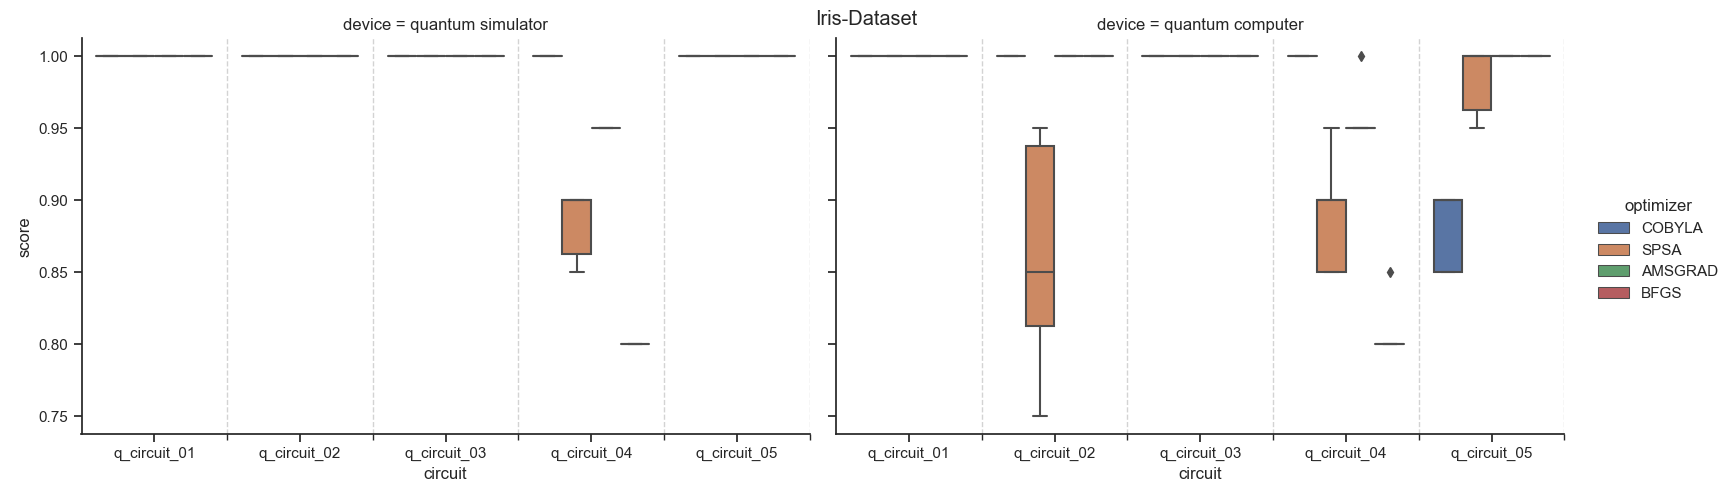
\includegraphics[width=1.0\linewidth]{thesis/Figures/qnn/boxplots/100_iris.png} 
        \label{subfigure:accuracy_comparison_boxplots_iris_dataset1}
    \end{subfigure}
    \\[-3ex]
    \begin{subfigure}{1.0\textwidth}
        \centering
        \subcaption{Rain}
        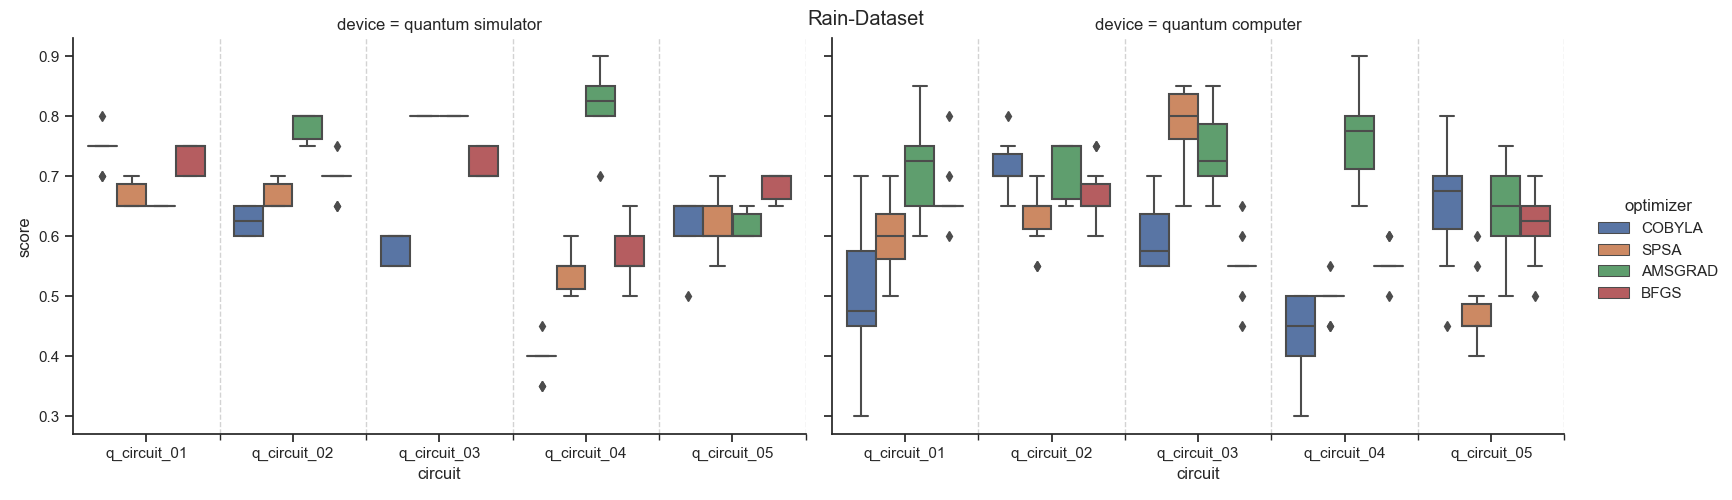
\includegraphics[width=1.0\linewidth]{thesis/Figures/qnn/boxplots/100_rain.png} 
        \label{subfigure:accuracy_comparison_boxplots_rain_dataset1}
    \end{subfigure}
    \\[-3ex]
    \begin{subfigure}{1.0\textwidth}
        \centering
        \subcaption{Vlds}
        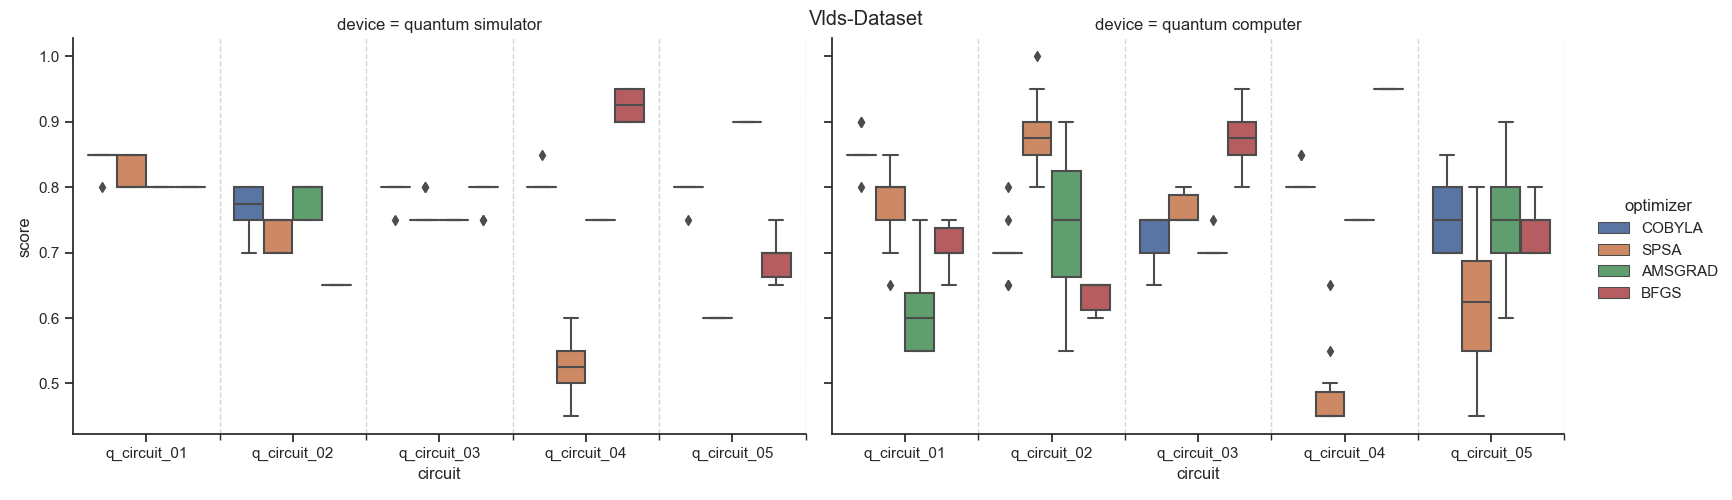
\includegraphics[width=1.0\linewidth]{thesis/Figures/qnn/boxplots/100_vlds.png} 
        \label{subfigure:accuracy_comparison_boxplots_vlds_dataset1}
    \end{subfigure}
    \\[-3ex]
    \begin{subfigure}{1.0\textwidth}
        \centering
        \subcaption{Custom}
        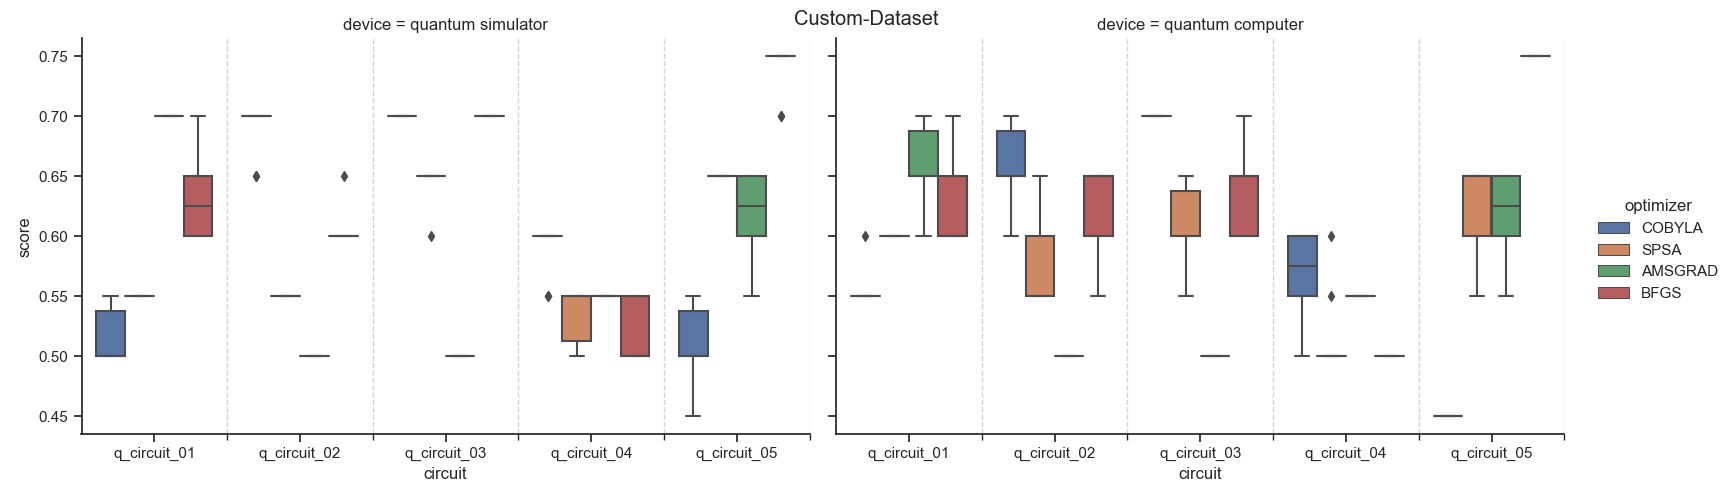
\includegraphics[width=1.0\linewidth]{thesis/Figures/qnn/boxplots/100_custom.png}
        \label{subfigure:accuracy_comparison_boxplots_custom_dataset1}
    \end{subfigure}
    \\[-3ex]
    \begin{subfigure}{1.0\textwidth}
        \centering
        \subcaption{Adhoc}
        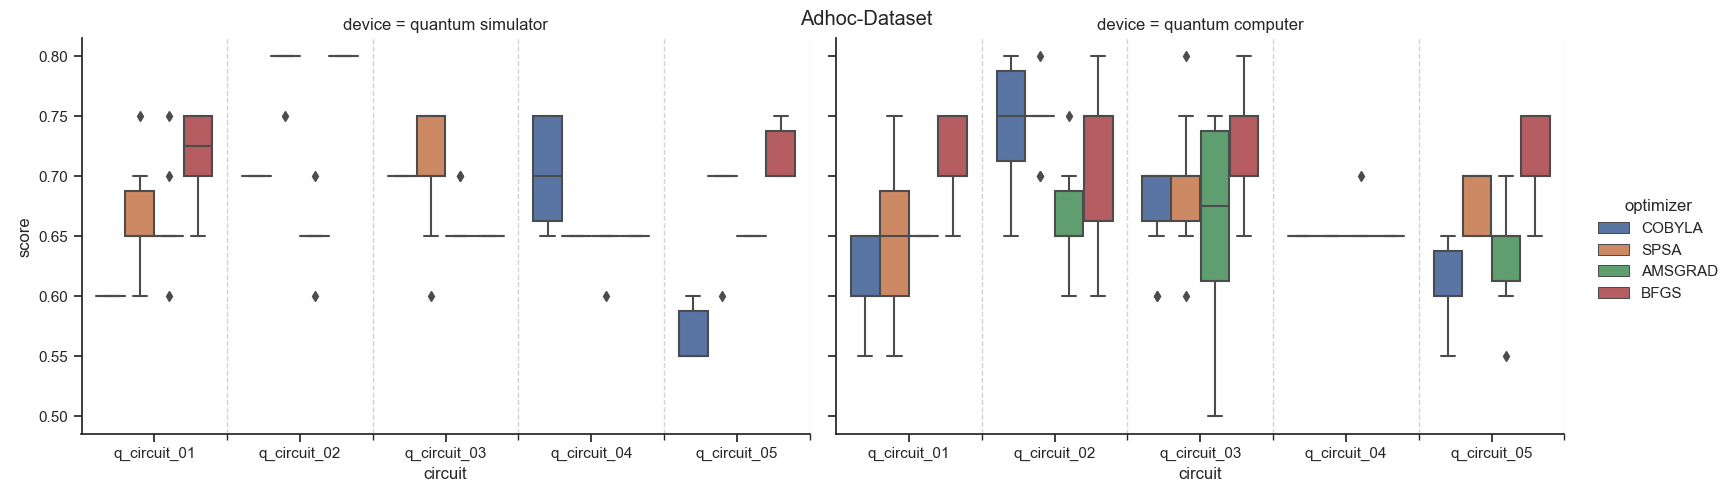
\includegraphics[width=1.0\linewidth]{thesis/Figures/qnn/boxplots/100_adhoc.png}
        \label{subfigure:accuracy_comparison_boxplots_adhoc_dataset1}
    \end{subfigure}
    \\[-3ex]
    \caption{Average accuracy comparison of 10 runs on the quantum simulator and computer for all binary datasets, circuits and optimizers.}
    \label{figure:accuracy_comparison_boxplots_binary_datasets}
\end{figure}


\clearpage

\subsubsection{Extended datasets}
\label{subsubsection:extended_datasets_comparison}
\begin{table}[!h]
	\centering
	\begin{tabular}{r|cc|cc}
		\hline 
		\thead{Dataset} & \thead{QNN\\(Simulator)} & \thead{QNN\\(Computer)} & \thead{QSVM\\(Simulator)} & \thead{QSVM\\(Computer)} \\
		\hline 
		Iris    & 0.933 & 0.943 & -  & - \\
		Rain    & 0.690 & 0.530 & -  & - \\
		Vlds    & 0.863 & 0.560 & -  & - \\
		Custom  & 0.549 & 0.557 & -  & - \\
		Adhoc   & 0.603 & 0.566 & -  & - \\
		\hline
		\textbf{Average}  & \textbf{0.728} & \textbf{0.631} & \textbf{-} & \textbf{-}  \\
		\hline
	\end{tabular}
	\caption{Comparison of the QNN and QSVM accuracy on a quantum simulator as well as on a real quantum computer. The table shows the accuracy of the best approach for each of the VQCs and optimizer types using the extended datasets. The QSVM results have not been available at the time of writing.}
	\label{table:comparison_extended_datasets_accuracy}
\end{table}

\clearpage

\subsection{Comparison between QNN and QSVM}
According to Havlicek et al. the the generic decision function of an SVM classifier as seen in equation \ref{equation:svm_decision_function} has the same form as the decision function from a QNN seen in equation \ref{equation:qnn_decision_function}, therefore, the QNN implements a linear decision boundary in feature space\cite{havlicekSupervisedLearningQuantum2019}. \textit{Note: The equasions \ref{equation:svm_decision_function}, \ref{equation:qnn_decision_function}, \ref{equation:w_alpha_real_coefficient}, \ref{equation:psi_alpha_real_coefficient} and the descriptions between them have been taken from \cite{ThomsenComparingQNNs_QSVM}}.

\begin{equation}
    \centering
        \tilde{c}_{SVM}(\mathbf{x}) =\ sign[\ip{\Vec{w}}{\phi(\mathbf{x})}_{\mathcal{H}}+b]
    \label{equation:svm_decision_function}
\end{equation}

with $\mathbf{x}$ as input data vector in the original space $\mathbb{R}^s$ and where $\Vec{w} \in \mathcal{H}$ and $\ip{\cdot}{\cdot}_{\mathcal{H}}$ as inner product of $\mathcal{H}$ and $\mathcal{H}$ is a possibly infinite dimensional Hilbert space. Here the notation $\Vec{w}$ is for vectors in the Hilbert/feature space. Bias is defined as $b \in [−1, +1]$

\begin{equation}
    \centering
        \tilde{c}_{QNN}(\mathbf{x}) =\ sign[\frac{1}{2^q} \sum_{\alpha} w_{\alpha}(\theta)\psi_{\alpha}(\mathbf{x})+b]
    \label{equation:qnn_decision_function}
\end{equation}

where $w_{\alpha}(\theta)$ and $\psi_{\alpha}(\mathbf{x})$ are real coefficients defined as

\begin{equation}
    \centering
        w_{\alpha}(\theta) =\ tr[\mathcal{W}(\theta)^{\dag}\mathcal{F}\mathcal{W}(\theta)\mathcal{P}_{\alpha}]\footnotemark[1]
    \label{equation:w_alpha_real_coefficient}
\end{equation}

and 

\begin{equation}
    \centering
        \psi_{\alpha}(\mathbf{x}) =\ tr[\op{\psi(\mathbf{x})}{\psi(\mathbf{x})}\mathcal{P}_{\alpha}]\footnotemark[1]
    \label{equation:psi_alpha_real_coefficient}
\end{equation}

\footnotetext[1]{We refer the reader to the papers \cite{havlicekSupervisedLearningQuantum2019,ThomsenComparingQNNs_QSVM} for the definition of $\mathcal{P}_{\alpha}$.}

The same is concluded by M. Schuld as seen in the illustration \ref{figure:2101.11020_Maria_Schuld_Fig.3} taken from her paper \cite{schuld_SQMLmodelsAreKernelMethods} while stating: 
\begin{displayquote}
"The bridge between quantum machine learning and kernel methods is formed by the observation that quantum models map data into a high-dimensional feature space, in which the measurement defines a linear decision boundary."
\end{displayquote}

\begin{figure}[!h]
    \centering
    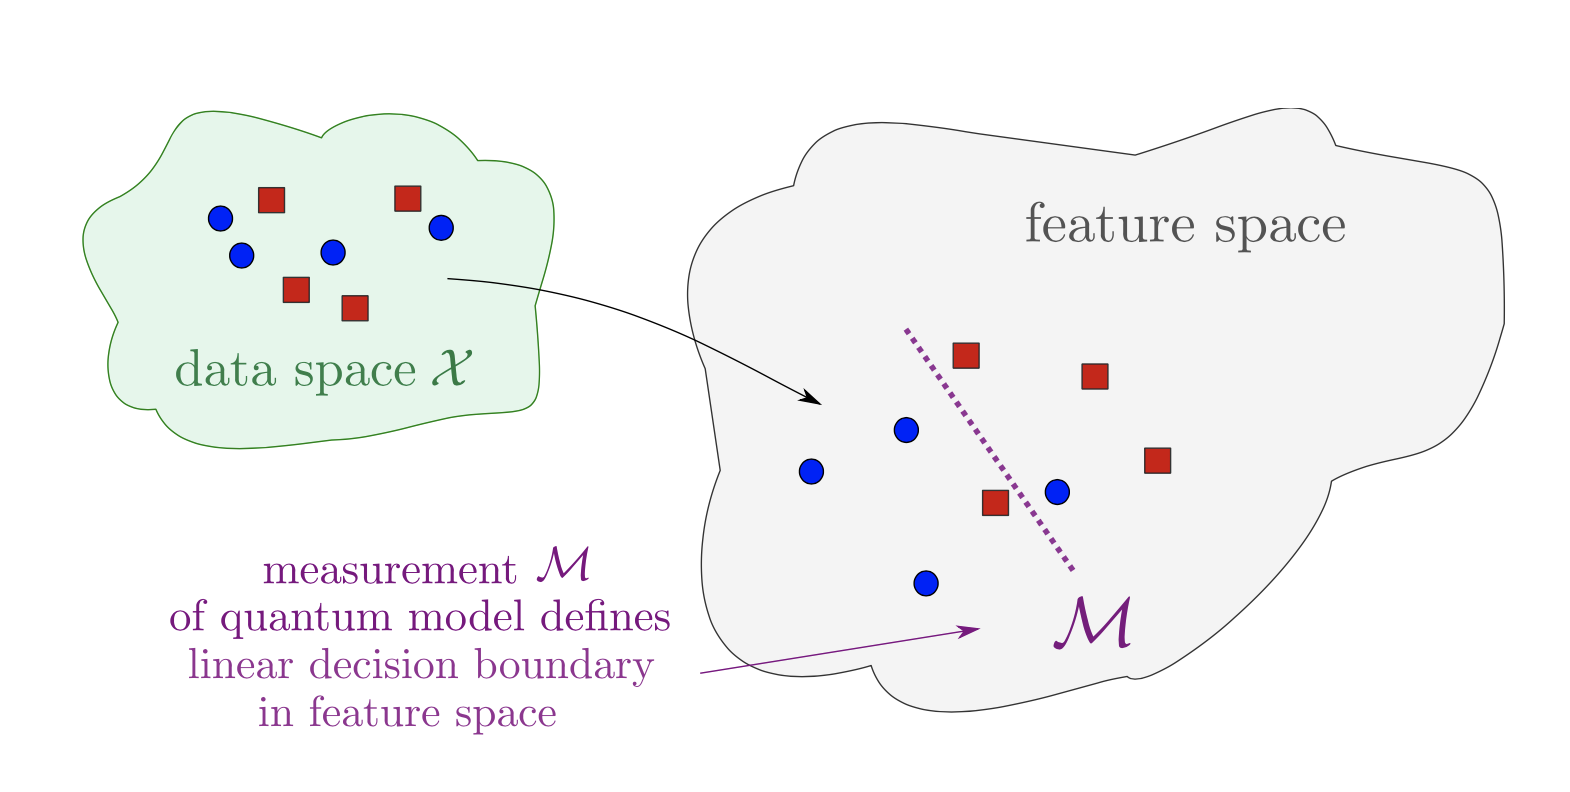
\includegraphics[width=0.7\linewidth]{thesis/Figures/qnn/2101.11020_Maria_Schuld_Fig.3.png} 
    \caption{\textbf{Quantum models as linear models in a feature space}. A quantum model can be understood as a model that maps data into a feature space in which the measurement defines a linear decision boundary. This feature space is not identical to the Hilbert space of the quantum system. Instead we can define it as the space of complex matrices enriched with the Hilbert-Schmidt inner product – which is the space where density matrices live in.\cite{schuld_SQMLmodelsAreKernelMethods}}
    \label{figure:2101.11020_Maria_Schuld_Fig.3}
\end{figure}

While QNN and QSVM both implement a linear decision boundary in the feature space the main difference lies in the variational circuit $\mathcal{W}(\theta)$ as seen in figure \ref{fig:general_structure_qsvm_and_qnn}.

\begin{figure}[!ht]
    \centering
    \begin{subfigure}{1.0\textwidth}
        \centering
	    \scalebox{0.8}{
        \Qcircuit @C=1.4em @R=0.8em {
                & & \ket{\psi(\vec{x_i})} & & & \\
                & & & & & & \\
                \lstick{\ket{0}} & \multigate{3}{\qquad\mathcal{E}(\Vec{x_i})\qquad} \barrier[0em]{3} & \qw       & \multigate{3}{\qquad \mathcal{E}(\Vec{x_j})^{\dag} \qquad} & \meter \\
                \lstick{\ket{0}} & \ghost{\qquad\mathcal{E}(\Vec{x_i})\qquad}                         & \qw       & \ghost{\qquad \mathcal{E}(\Vec{x_j})^{\dag} \qquad}        & \meter \\
                \vdots           & \nghost{\qquad\mathcal{E}(\Vec{x_i})\qquad}                        & \nghost{} & \nghost{\qquad \mathcal{E}(\Vec{x_j})^{\dag} \qquad}       & \vdots \\
                \lstick{\ket{0}} & \ghost{\qquad\mathcal{E}(\Vec{x_i})\qquad}                         & \qw       & \ghost{\qquad \mathcal{E}(\Vec{x_j})^{\dag} \qquad}        & \meter \\
                & & & & & & \\
            }
    	}
    	\subcaption{General quantum circuit structure of a QSVM kernel estimator with a parametrized unitary $\mathcal{E}(\Vec{x_i})$ followed by its adjoint $\mathcal{E}(\Vec{x_j})^{\dag}$. The kernel can only be evaluated approximately with a finite number of measurement shots due to the probalistic nature of quantum computing.}
    	\label{subfigure:general_structure_qsvm}
    \end{subfigure}
    \\[2em]
    \begin{subfigure}{1.0\textwidth}
        \centering
	    \scalebox{0.8}{
        \Qcircuit @C=1.4em @R=0.8em {
                & & \ket{\psi(\vec{x})} & & & \\
                & & & & & & \\
                \lstick{\ket{0}} & \multigate{3}{\qquad\mathcal{U}_{\Phi(\Vec{x})}\qquad} \barrier[0em]{3} & \qw       & \multigate{3}{\qquad W(\theta) \qquad} & \meter \\
                \lstick{\ket{0}} & \ghost{\qquad\mathcal{U}_{\Phi(\Vec{x})}\qquad}                         & \qw       & \ghost{\qquad W(\theta) \qquad}        & \meter \\
                \vdots           & \nghost{\qquad\mathcal{U}_{\Phi(\Vec{x})}\qquad}                        & \nghost{} & \nghost{\qquad W(\theta) \qquad}       & \vdots \\
                \lstick{\ket{0}} & \ghost{\qquad\mathcal{U}_{\Phi(\Vec{x})}\qquad}                         & \qw       & \ghost{\qquad W(\theta) \qquad}        & \meter \\
                & & & & & & \\
            }
    	}
        \subcaption{General quantum circuit structure of a QNN, which is defined to consist of a feature map circuit $\mathcal{U}_{\Phi(\Vec{x})}$ followed by a variational form circuit $W(\theta)$ strictly separating the fixed input vector $\Vec{x}$ and trainable parameters $\theta$.}
    	\label{subfigure:general_structure_qnn}
    \end{subfigure}
    \caption{General schematics of a variational quantum circuit and quantum support vector machine circuit.}
    \label{fig:general_structure_qsvm_and_qnn}
\end{figure}

Thomsen further states the following: 

\begin{displayquote}
"The main difference between the QNN and QSVM now lies in the parameterized coefficients $w_{\alpha}(\theta)$ that make up the vector $w(\vec{\theta}) \in \mathcal{S}(\mathcal{H}_2^{\otimes n})$ that defines the direction of the hyperplane in feature space according to which class membership is assigned by the QNN. Because these coefficients are determined through a variational circuit $W(\theta)$, they can not take on arbitrary values in general. In particular, there is no guarantee that the solution to the dual QSVM optimization problem in (2.17) on page 12 denoted by $\vec{w}^*$ is accessible to the QNN. But $\vec{w}^*$ is guaranteed to be found by the QSVM due to convexity and guaranteed to maximize the (regularized by slack) margin in feature space by strong duality. With this, the QNN can be interpreted as an approximation to the QSVM that finds a solution that is at best equally good, depending on the expressivity of the variational form."\footnote[1]{The mentioned optimization problem equation 2.17 does not contain the denoted $\vec{w}^*$ which may is a reference error and thus has been omitted in this thesis.}
\end{displayquote}

\clearpage

Again we can compare this to the findings of M. Schuld in the same paper mentioned above by studying the caption and illustration which can be seen in figure \ref{figure:2101.11020_Maria_Schuld_Fig.5}.

\begin{figure}[!h]
    \centering
    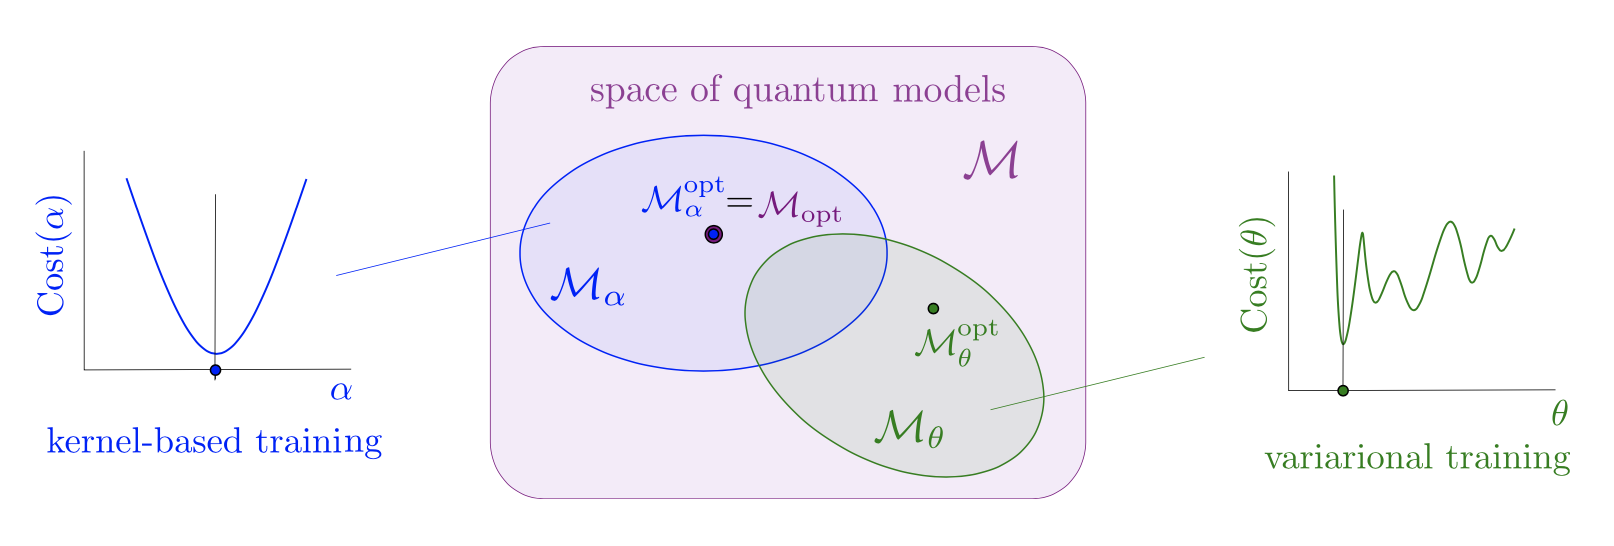
\includegraphics[width=1.0\textwidth]{thesis/Figures/qnn/2101.11020_Maria_Schuld_Fig.5.png} 
    \caption{\textbf{Kernel-based training vs. variational training}. Training a quantum model as defined here tries to find the optimal measurement Mopt over all possible quantum measurements. Kernel theory guarantees that in most cases this optimal measurement will have a representation that is a linear combination in the training data with coefficients $\alpha = (\alpha_1,...,\alpha_M)$. Kernel-based training therefore optimises over the parameters $a$ directly, effectively searching for the best model in an M-dimensional subspace spanned by the training data (blue). We are guaranteed that $M_{\alpha}^{opt} = M_{opt}$, and if the loss is convex $\alpha$ this is the only minimum, which means that kernel-based training will find the best measurement out of all measurements. Variational training parametrises the measurement instead by a general ansatz that depends on $K$ parameters $\theta = (\theta_1,...,\theta_K)$, and tries to find the optimal measurement $M_{\theta}^{opt}$ in the subspace explored by the ansatz. This $\theta$-subspace is not guaranteed $\theta$ to contain the globally optimal measurement $M_{opt}$, and optimisation is usually non-convex. We are therefore guaranteed that kernel-based training finds better or the same minima to variational training, but at the expense of having to compute pairwise distances of data points for training and classification.\cite{schuld_SQMLmodelsAreKernelMethods}}
    \label{figure:2101.11020_Maria_Schuld_Fig.5}
\end{figure}

We can now finally conclude that the variational model of a QNN is the main difference and is not guaranteed to find the optimal measurement and is searching in a different subspace than the kernel-based QSVM. 

